% Gemini theme
% https://github.com/anishathalye/gemini

\documentclass[final]{beamer}

% ====================
% Color options
% ====================

\newif\ifgrayhighlight % define new flag
% \grayhighlighttrue     % Use gray background for highlighted block
\grayhighlightfalse    % Use cardinal red background for highlighted block

% ====================
% Packages
% ====================

\usepackage[T1]{fontenc}
\usepackage{lmodern}
\usepackage[size=custom,width=120,height=120,scale=1.0]{beamerposter}
\usetheme{gemini}
\usecolortheme{stanford}
\usepackage{graphicx}
\usepackage{booktabs}
\usepackage{tikz}
\usepackage{pgfplots}
\pgfplotsset{compat=1.14}
\usepackage{anyfontsize}

% ====================
% Lengths
% ====================

% If you have N columns, choose \sepwidth and \colwidth such that
% (N+1)*\sepwidth + N*\colwidth = \paperwidth
\newlength{\sepwidth}
\newlength{\colwidth}
\setlength{\sepwidth}{0.025\paperwidth}
\setlength{\colwidth}{0.3\paperwidth}

\newcommand{\separatorcolumn}{\begin{column}{\sepwidth}\end{column}}

% ====================
% Title
% ====================

\title{Software Best Practices for Reproducible Open Science}

\author{Alex Koufos (he/him)\inst{1}} %\and Ben Bitdiddle \inst{1}}

\institute[shortinst]{\inst{1} Stanford University}

% ====================
% Footer (optional)
% ====================

\footercontent{
  \href{https://github.com/exoticdft}{https://github.com/exoticdft} \hfill
  TESS/SPD 2024 - Dallas, TX --- 211-040 \hfill
  \href{mailto:akoufos@sun.stanford.edu}{akoufos@sun.stanford.edu}
}
% (can be left out to remove footer)

% ====================
% Logo (optional)
% ====================

% use this to include logos on the left and/or right side of the header:
\logoleft{
\includegraphics[height=3cm]{logos/stanford+solar_group+HEPL-white.pdf}}
\logoright{
\includegraphics[height=7cm]{logos/SUTree-2color.pdf}}

% ====================
% Body
% ====================

\begin{document}

\begin{frame}[t]
\begin{columns}[t]
\separatorcolumn

\begin{column}{\colwidth}

  \begin{block}{Is there a "reproducibility crisis" in the sciences?}

    Over the past two decades, many researchers have been discussing the
    potential issue within the whole of the science communities related to the
    ability to reproduce the scientific work of others, and even themselves.
    This issue has been termed the "Reproducibility Crisis" in the sciences.
    A recent Nature article\cite{baker2016} discusses this issue.
       
    \begin{figure}
      \centering
      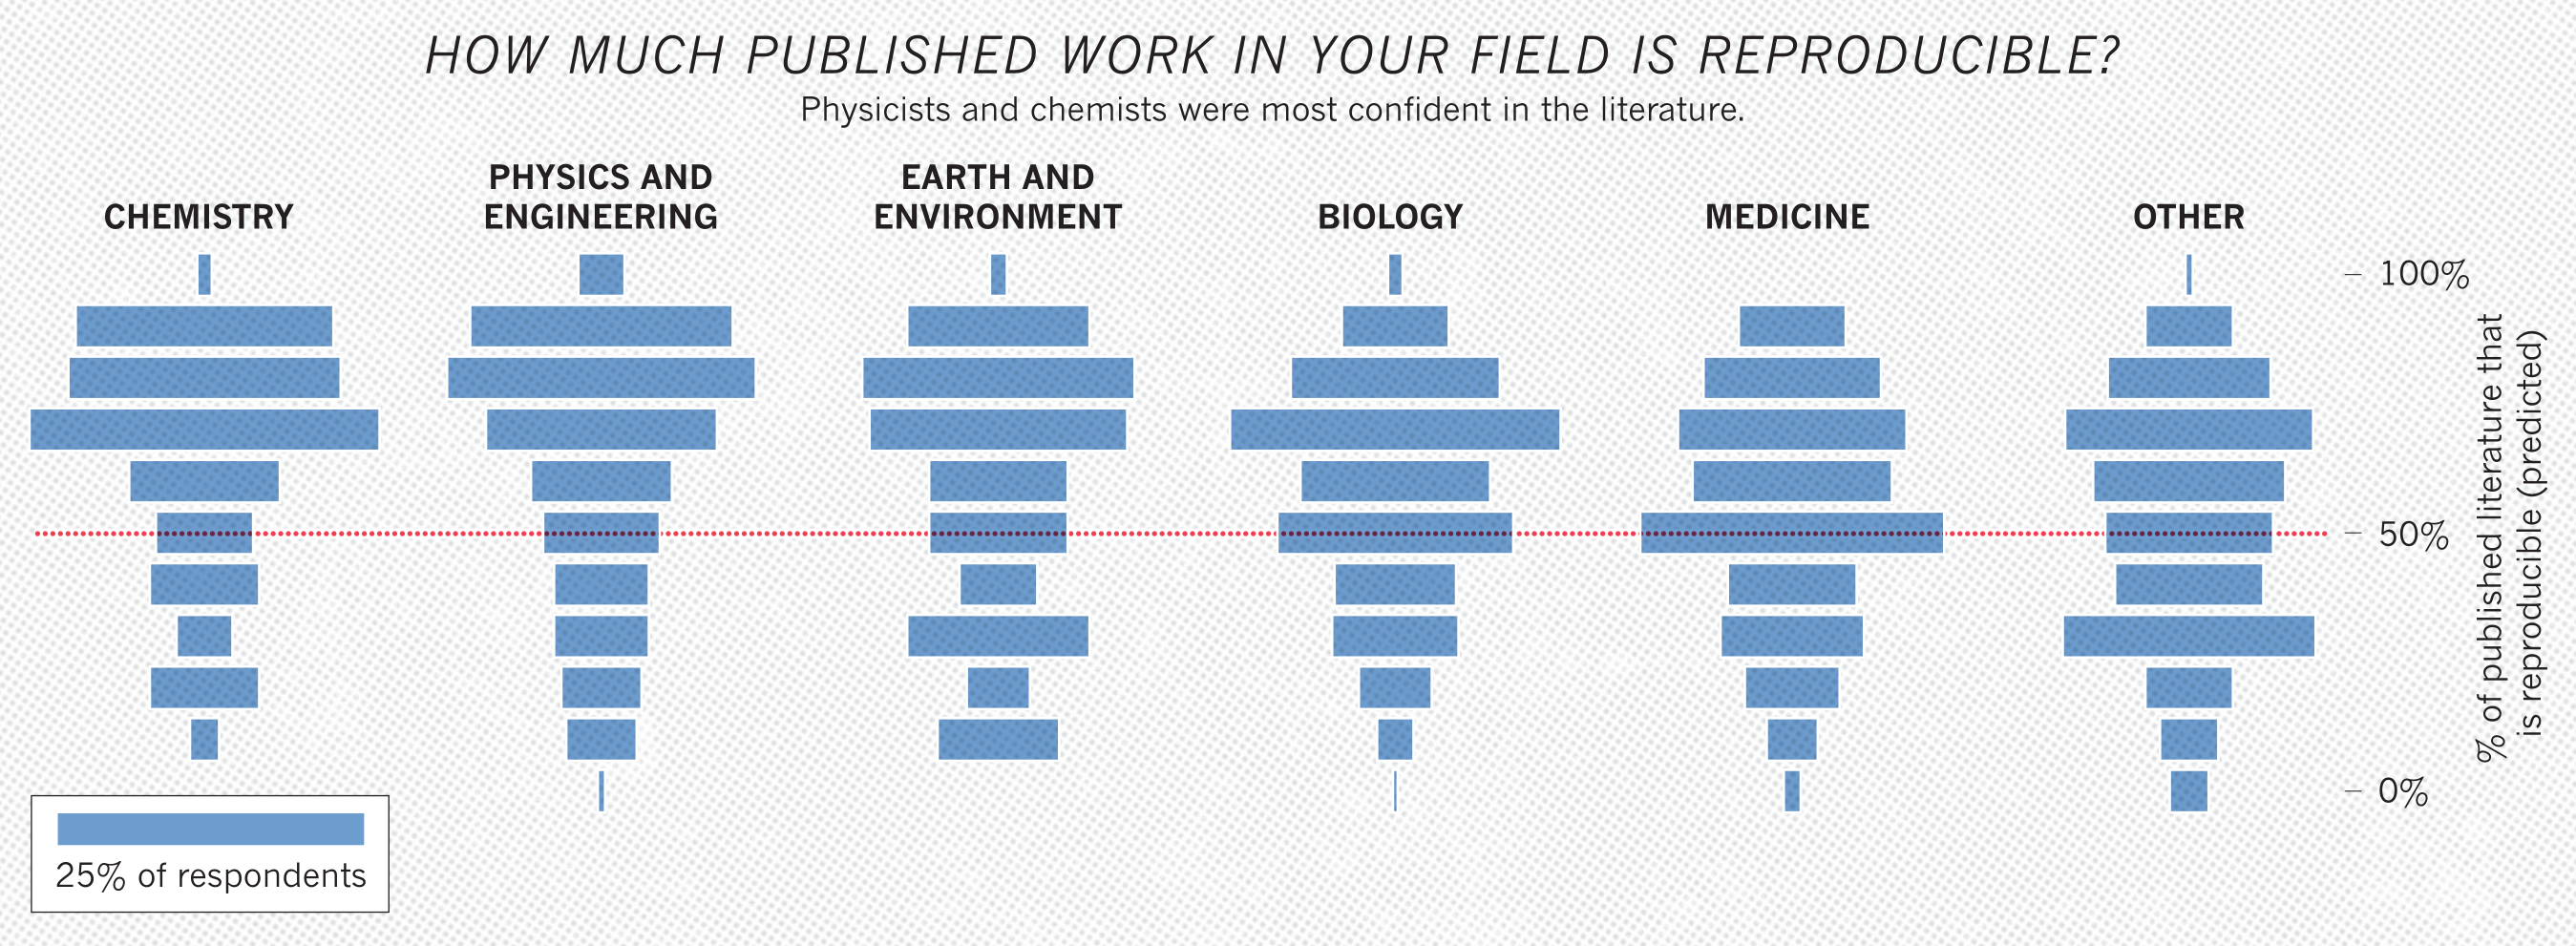
\includegraphics[width=0.85\textwidth]{tess2024/Nature-Field-Confidence.png}
      \caption{Science Field Based Confidence in Published Work (Baker, M. 2016)}
      \label{fig:confidence}
    \end{figure}

    Figure \ref*{fig:confidence} shows the general concern from those in the
    scientific community.
    In general, the physics and engineering community tends to be more
    confident in published literature.
    However, the research suggest there are still many researchers who are not
    confident.
    This issue leads to a lack of confidence from the general public.

    \begin{figure}
      \centering
      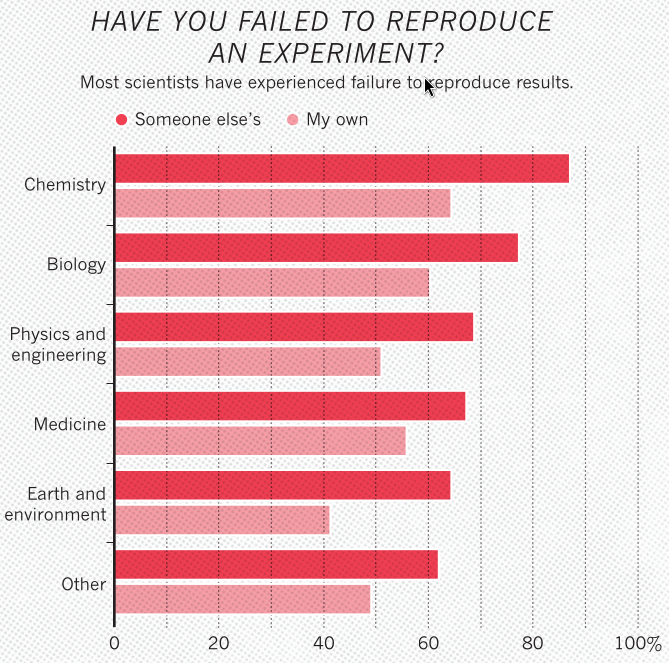
\includegraphics[width=0.85\textwidth]{tess2024/Nature-Reproducibility-Failure-.png}
      \caption{Failure to Reproduce Published Results (Baker, M. 2016)}
      \label{fig:failure}
    \end{figure}
    
    Figure \ref*{fig:failure} provides another metric for understanding this
    crisis.
    In all research communities, many researchers struggled to reproduce the
    results of others, and even themselves.
    This included the physics and engineering communities.

  \end{block}

  \begin{alertblock}{A Failure to Reproduce}
    Several reports have suggested there is a problem with researchers being
    able to reproduce their own work.
    The numbers suggest \textbf{over 50\% of the physics and engineering community
    were unable to reproduce their own work!}

  \end{alertblock}

  \begin{block}{But what is Reproducibility?}
    In 2019, a National Academy of Sciences committee exploring the
    reproducibility and replicability in scientific and engineering research.
    The committee define\cite{reproducibility_in_science}
    \begin{description}
      \item[reproducibility (i.e. computational reproducibility)] \hfill \\
      as obtaining consistent computational results using the same input data,
      computational steps, methods, code, and conditions of analysis
      \item[replicability] \hfill \\
      as obtaining consistent results across studies aimed at answering the same
      scientific question, each of which has obtained its own data
    \end{description}

    This poster will focus on the former definition.
    There are many techniques we can all use to help alleviate potential issues
    with being able to reproduce results.

  \end{block}

\end{column}

\separatorcolumn

\begin{column}{\colwidth}

  \begin{exampleblock}{Ways to help mitigate the reproducibility in your research}

    Software is essential and inherit in every aspect of modern research.
    The coding we do for this research is often overlooked as software
    engineering.
    However, we can learn a lot from the software engineering community and
    in the recent years there has been an emergence of associations focused on 
    "research software engineering (RSEng)", specifically.
    One such organization is the
    (\href{https://us-rse.org}{United States Research Software Engineer Association (US-RSE)})
    (several others are mentioned in the references section.)
    These communities strive to promote scientific software best practices to
    support better research.
    For example, the Better Scientific Software (BSSw)\cite{bssw} provides many
    resources, such as
    \href{https://bssw.io/items?topic=reproducibility}{https://bssw.io/items},
    to help researchers and RSEs create successful research projects.

    Although these resources can be extremely useful, their are a large amount
    of "best practices" one can use.
    So I'm going to discuss some of the "easier" and possibly more impactful
    tools one can use.
    I will focus on \textbf{version control}, \textbf{code reviews},
    \textbf{documentation}, and \textbf{testing}.
    
    Focusing some effort on these best practices can help with:
    \begin{itemize}
      \item Higher \textbf{reusability} of code (less need to copy and paste
        things that already work)
      \item Better \textbf{reproducibility} and \textbf{robustness} of software
        (verify/validate results and handle errors)
      \item Improved \textbf{scalability} (ability to add new features and
        complexity)
      \item Enhanced \textbf{collaboration} (work with others)
      \item Boosted \textbf{clarity} (reminders of what you did and helps other
        follow)
      \item Greater \textbf{transferability} of data and programs (work
        anywhere, sharing, etc.)
      \item \textbf{Transparency} of results and methods (helps public trust
        and explaining to others)
    \end{itemize}
    
    \textbf{Disclaimer:} None of the these techniques can single handedly
    resolve, or entirely mitigate the problem of reproducibility.
    However, together they can help reduce unintended difficulties for others,
    or even yourself, in reproducing your work in the future.

  \end{exampleblock}

  \begin{block}{Best Practice: Version Control}

    \heading{What is version control?}
    Version control can be an extremely useful tool to track changes to your
    software (and experimentation) throughout your research endeavor.
    If you are unfamiliar with version control tools, you probably have used
    some system yourself for tracking your changes.
    For example,
    \href{https://phdcomics.com/comics/archive.php?comicid=1531}{PhD Comics}
    jokes about a common practice many of us (myself included) have used in the
    past to track our research papers, where you simply save a new file with
    changes from the last iteration and name it `whatever-rev2.doc`.
    This of course can get quite tenuous quickly when you have 10+ revisions.
    \\ \vspace{1em}
    \textbf{Protip:} Check out \href{overleaf.com}{overleaf.com} for tracking
    document changes if working with LaTeX.
    \\ \vspace{1em}
    This history of these changes (and all its metadata) is called a
    "repository" or "repo".
    Version control is essentially a history of snapshots of your software.

    \heading{Why use version control?}
    Version control can help with \textbf{reproducibility},
    \textbf{robustness}, \textbf{scalability}, \textbf{transparency}, and
    \textbf{collaboration}.

    \heading{How you can use version control}
    When working with software, \href{https://git-scm.com/}{Git} is one of the
    most popular tools for version control.
    It ties directly into management software, such as
    \href{https://github.com}{GitHub} and \href{https://gitlab.com}{GitLab}.
    This is done by saving just the changes between snapshots as "commits" in
    a linked list, often visualized as a directional acyclic graph.
    Figure \ref{fig:git-simple} and \ref{fig:git-github-flow} show the history
    of two different Git repositories.
    These type of diagrams are general known as "commit graphs".
    
    In both these figures, commits are shown as circles, with directional lines
    referencing a previous commit, like a linked list.
    Each commit contains the changes since the last commit (its parent node),
    thus tracking the history of the repo over time.
    This allows us to easily understand and compare changes between versions.
    People like to refer to these commit graphs like trees, with a trunk and
    branches off the trunk.

    \begin{figure}
      \centering
      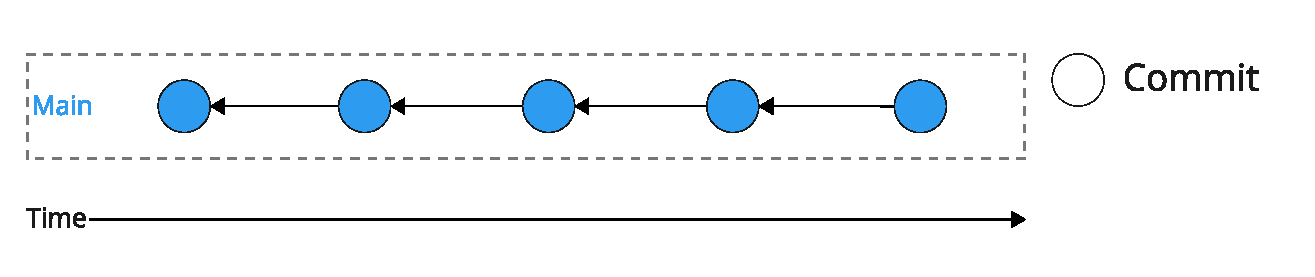
\includegraphics[width=0.95\textwidth]{tess2024/git-simple-git-repo.pdf}
      \caption{Version Control: A simple Git history of the "main" branch}
      \label{fig:git-simple}
    \end{figure}

    Figure \ref*{fig:git-simple} shows the simplest way to use Git.
    In the figure we see just 5 commits starting from the left to the right.
    Each commit represents a snapshot of the repo at that moment in time,
    compared against the previous commit (the very first commit or snapshot
    is considered empty.)
    So, in this commit graph, we are simply committing each of our changes
    against the "main" branch, i.e. the trunk.

    \begin{figure}
      \centering
      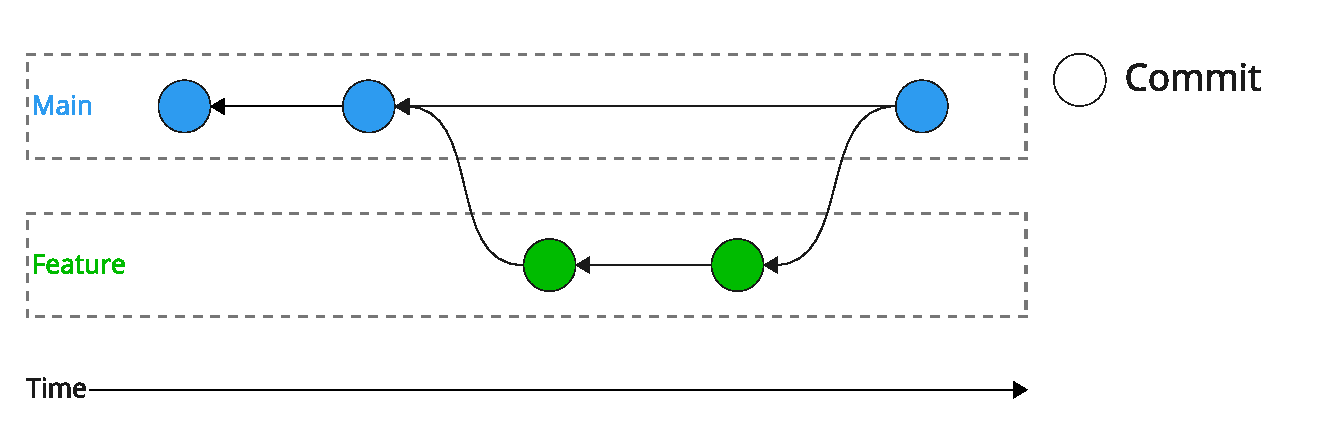
\includegraphics[width=0.95\textwidth]{tess2024/git-github-flow.pdf}
      \caption{Version Control: A Git repo using a branching model known as
        GitHub Flow}
      \label{fig:git-github-flow}
    \end{figure}

    Figure \ref*{fig:git-github-flow} shows a slightly more involved way of
    tracking changes known as the "GitHub Flow" workflow or "branching model".
    A branching model is simple a plan for managing and tracking your changes
    over time.
    Here the "main" branch or trunk is generally considered a stable branch;
    meaning the branch will attempt to only contain working, verified software,
    while the branches off of this trunk are work in progress changes.
    
    % Let's consider a really basic example of using this model.
    % One could imagine a code base with a script that prints some message, let's
    % say "Hello world!", to the screen.
    % The first commit, i.e. "initial commit", is just this simple script with
    % the functionality to print your message.
    % You add to the script an addition part of the message "Have a wonderful
    % day!" and commit this change to the main branch.
    % Now, you want to add new functionality (or feature) to your script to get
    % the name of the person calling your script.
    % Instead of committing directly to the main branch, which you know works, you
    % can make a branch off of main and begin adding your changes.
    % On this new branch, let's call it "feature", you add the ability to get user
    % input and update the message to "Hello World! Have a wonderful day,
    % \textit{User}!", then you commit on this new branch.
    % However, after making your commit, you realize there is an issue where the
    % user can provide anything as input, so you refine the input request to be
    % more specific and commit this change.
    % Once you are satisfied the new functionality is doing what you desire, you
    % finalize this branch by "merging" the changes back into the main branch.
    % Now, your main branches history will see these two commits as a single
    % set of changes against its previous stable commit.
    % In other words, the main branch will seem to have three commits in its
    % history all which work in a stable way.

  \end{block}

\end{column}

\separatorcolumn

\begin{column}{\colwidth}

  \begin{block}{Best Practice: Code Reviews}

    \heading{What are code reviews?}
    Code reviewing, simply put, is a process in which you, or others, look over
    the changes to your code (or repo) over some period of time.
    Essentially, having a second look at your changes.
    Generally, this is done at the end of (but sometimes during) a specific set
    of changes to the code base.
    These sets of changes are usually associated with a request for new
    functionality, resolving a known bug, updating existing functionality, or
    really anything you'd like.
  
    \heading{Why use code reviews?}
    Incorporating this process can be really helpful to catch bugs before they
    are added to stable code, or just used as a way to share how software works
    with team members.
    Code reviews can help with \textbf{reproducibility},
    \textbf{robustness}, \textbf{clarity}, \textbf{transferability}, and
    \textbf{collaboration}.
  
    \heading{How you can use code reviews}
    Code review is one of the more involved processes, as it requires not only
    tool, but a standardize procedure to try to follow.
    For each team, this will likely be different.
    However, there are several resources you can reference to learn more.
    Here I briefly talk about the use of a process known as "pull requests" or
    "merge requests".
    This process is generally directly implemented by repo management tools I
    mentioned earlier, such as GitHub and GitLab.
    In general, the process is three or four steps:
    1. Update your codes (i.e. make changes), 2. Use a tool to review older
    and newer files (i.e. review changes), 3. Make suggestions and comments
    (discuss changes) and repeat, and 4. Merge changes into stable code.
    Figure \ref*{fig:code-review} show the flow diagram of this process, with
    the option of discussing changes when the initial code changes might not be
    adequate.

    \begin{figure}
      \centering
      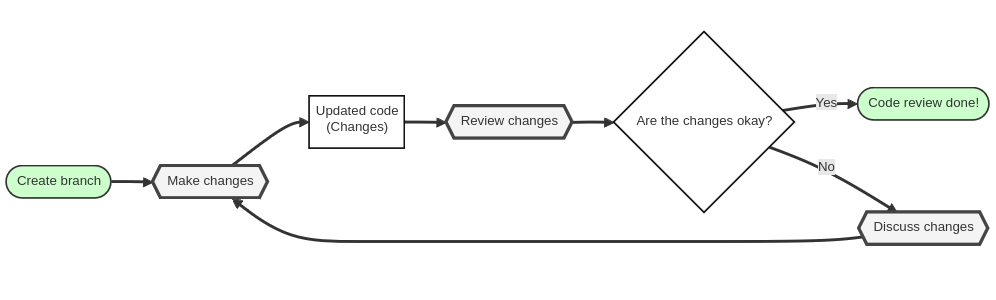
\includegraphics[width=0.95\textwidth]{tess2024/code-review-flow-diagram.png}
      \caption{Code Review: The basic code review process}
      \label{fig:code-review}
    \end{figure}
    
    GitHub has a built-in system for doing these code reviews.
    However, you can implement the process without it, GitHub and GitLab, just
    make it easier.
    You will need to learn a bit of GitHub to do the process, but you'd have to
    do the same if you implement your own.
    If you decide to use GitHub, there are many useful resouces online to learn
    and practice the process before implementing on important code.
    For example, an interactive tutorial can be found at
    \href{https://code-review.org}{code-review.org}.

  \end{block}

  \begin{block}{Best Practice: Documentation}

    Class aptent taciti sociosqu ad litora torquent per conubia nostra, per
    inceptos himenaeos. Phasellus libero enim, gravida sed erat sit amet,
    scelerisque congue diam. Fusce dapibus dui ut augue pulvinar iaculis.

    \begin{table}
      \centering
      \begin{tabular}{l r r c}
        \toprule
        \textbf{First column} & \textbf{Second column} & \textbf{Third column} & \textbf{Fourth} \\
        \midrule
        Foo & 13.37 & 384,394 & $\alpha$ \\
        Bar & 2.17 & 1,392 & $\beta$ \\
        Baz & 3.14 & 83,742 & $\delta$ \\
        Qux & 7.59 & 974 & $\gamma$ \\
        \bottomrule
      \end{tabular}
      \caption{A table caption.}
    \end{table}

    Donec quis posuere ligula. Nunc feugiat elit a mi malesuada consequat. Sed
    imperdiet augue ac nibh aliquet tristique. Aenean eu tortor vulputate,
    eleifend lorem in, dictum urna. Proin auctor ante in augue tincidunt
    tempor. Proin pellentesque vulputate odio, ac gravida nulla posuere
    efficitur. Aenean at velit vel dolor blandit molestie. Mauris laoreet
    commodo quam, non luctus nibh ullamcorper in. Class aptent taciti sociosqu
    ad litora torquent per conubia nostra, per inceptos himenaeos.

    Nulla varius finibus volutpat. Mauris molestie lorem tincidunt, iaculis
    libero at, gravida ante. Phasellus at felis eu neque suscipit suscipit.
    Integer ullamcorper, dui nec pretium ornare, urna dolor consequat libero,
    in feugiat elit lorem euismod lacus. Pellentesque sit amet dolor mollis,
    auctor urna non, tempus sem.

  \end{block}

  \begin{block}{Best Practice: Testing}

    Class aptent taciti sociosqu ad litora torquent per conubia nostra, per
    inceptos himenaeos. Phasellus libero enim, gravida sed erat sit amet,
    scelerisque congue diam. Fusce dapibus dui ut augue pulvinar iaculis.

    Donec quis posuere ligula. Nunc feugiat elit a mi malesuada consequat. Sed
    imperdiet augue ac nibh aliquet tristique. Aenean eu tortor vulputate,
    eleifend lorem in, dictum urna. Proin auctor ante in augue tincidunt
    tempor. Proin pellentesque vulputate odio, ac gravida nulla posuere
    efficitur. Aenean at velit vel dolor blandit molestie. Mauris laoreet
    commodo quam, non luctus nibh ullamcorper in. Class aptent taciti sociosqu
    ad litora torquent per conubia nostra, per inceptos himenaeos.

  \end{block}

  \begin{block}{References}

    \nocite{*}
    \footnotesize{\bibliographystyle{plain}\bibliography{poster}}

  \end{block}

\end{column}

\separatorcolumn
\end{columns}
\end{frame}

\end{document}
